% The Keccak state array [FIPS 202, §3.1.1, Figure 1]: 5 x 5 x w bits, with lanes along z,
% rows along x, columns along y, slices of constant z and planes of constant y.
% Original drawing for the Hash library.
\documentclass[tikz,border=6pt]{standalone}
\usepackage[T1]{fontenc}
\usepackage{lmodern}
\usepackage{amssymb}
% Shared style for the Hash diagrams.
% Palette: Okabe–Ito (colour-blind safe). Every diagram is drawn on an opaque white card so it
% stays legible on dark page themes.
\usetikzlibrary{arrows.meta,positioning,calc,fit,backgrounds}
\definecolor{hsblue}{HTML}{0072B2}
\definecolor{hsorange}{HTML}{E69F00}
\definecolor{hsgreen}{HTML}{009E73}
\definecolor{hsvermilion}{HTML}{D55E00}
\definecolor{hspurple}{HTML}{CC79A7}
\definecolor{hsink}{HTML}{1F2933}
\tikzset{
  >={Stealth[length=2.2mm]},
  every node/.style={font=\sffamily\small, text=hsink},
  wire/.style={draw=hsink, line width=0.6pt, ->},
  reg/.style={draw=hsink, line width=0.6pt, fill=hsblue!12, minimum width=9mm, minimum height=7mm},
  fn/.style={draw=hsink, line width=0.6pt, fill=hsorange!25, rounded corners=2pt, minimum width=10mm, minimum height=6mm},
  input/.style={draw=hsink, line width=0.6pt, fill=hsgreen!20, minimum width=9mm, minimum height=6mm},
  add/.style={circle, draw=hsink, line width=0.6pt, fill=white, inner sep=0pt, minimum size=5mm, font=\sffamily\bfseries},
  card/.style={fill=white, rounded corners=4pt},
}

\begin{document}
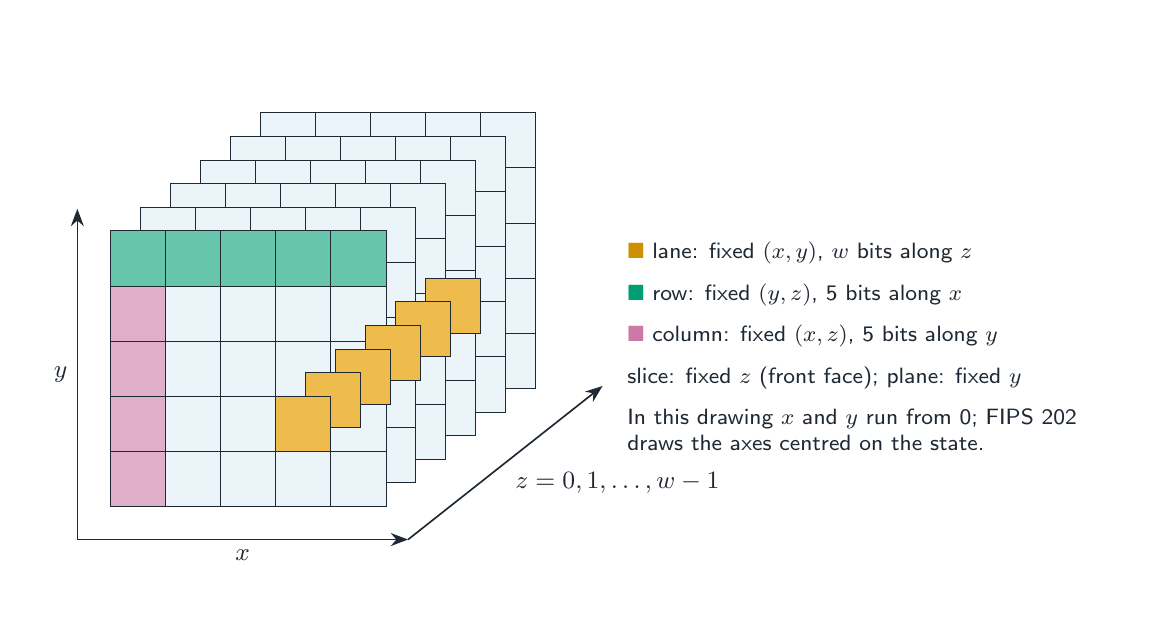
\begin{tikzpicture}[x={(0.7cm,0)}, y={(0,0.7cm)}, z={(0.38cm,0.3cm)},
    cell/.style={draw=hsink, line width=0.35pt}]
  % Slices z = 0, ..., 5 (front to back), each 5 x 5.
  \foreach \zz in {5,4,...,0} {
    \foreach \xx in {0,...,4} {
      \foreach \yy in {0,...,4} {
        \filldraw[cell, fill=hsblue!8] (\xx,\yy,\zz) -- ++(1,0,0) -- ++(0,1,0) -- ++(-1,0,0) -- cycle;
      }
    }
  }
  % A lane: x = 3, y = 1, all z (orange).
  \foreach \zz in {5,4,...,0} {
    \filldraw[cell, fill=hsorange!70] (3,1,\zz) -- ++(1,0,0) -- ++(0,1,0) -- ++(-1,0,0) -- cycle;
  }
  % A row: y = 4, z = 0 (green), and a column: x = 0, z = 0 (purple).
  \foreach \xx in {0,...,4} {
    \filldraw[cell, fill=hsgreen!60] (\xx,4,0) -- ++(1,0,0) -- ++(0,1,0) -- ++(-1,0,0) -- cycle;
  }
  \foreach \yy in {0,...,3} {
    \filldraw[cell, fill=hspurple!60] (0,\yy,0) -- ++(1,0,0) -- ++(0,1,0) -- ++(-1,0,0) -- cycle;
  }
  % Axes.
  \draw[wire] (-0.6,-0.6,0) -- node[below] {$x$} (5.4,-0.6,0);
  \draw[wire] (-0.6,-0.6,0) -- node[left] {$y$} (-0.6,5.4,0);
  \draw[wire] (5.4,-0.6,0) -- node[below right] {$z = 0, 1, \ldots, w-1$} (5.4,-0.6,6.5);
  % Legend.
  \node[anchor=west, font=\sffamily\footnotesize] (l1) at (9.2,4.6,0)
    {\textcolor{hsorange!90!black}{$\blacksquare$} lane: fixed $(x, y)$, $w$ bits along $z$};
  \node[anchor=north west, font=\sffamily\footnotesize] (l2) at (l1.south west)
    {\textcolor{hsgreen}{$\blacksquare$} row: fixed $(y, z)$, 5 bits along $x$};
  \node[anchor=north west, font=\sffamily\footnotesize] (l3) at (l2.south west)
    {\textcolor{hspurple}{$\blacksquare$} column: fixed $(x, z)$, 5 bits along $y$};
  \node[anchor=north west, font=\sffamily\footnotesize] (l4) at (l3.south west)
    {slice: fixed $z$ (front face); plane: fixed $y$};
  \node[anchor=north west, font=\sffamily\footnotesize, text width=6cm] (l5) at (l4.south west)
    {In this drawing $x$ and $y$ run from 0; FIPS 202 draws the axes centred on the state.};
  \begin{scope}[on background layer]
    \coordinate (e1) at (-1.2,-1.6,0);
    \coordinate (e2) at (5.6,5.6,6.5);
    \node[card, fit=(e1)(e2)(l1)(l5), inner sep=6pt] {};
  \end{scope}
\end{tikzpicture}
\end{document}
